% Figures for the conference version (two-column IEEE). Each is a macro called once, next to the text that first discusses it.
\newcommand{\figArch}{\begin{figure*}[!t]
\centering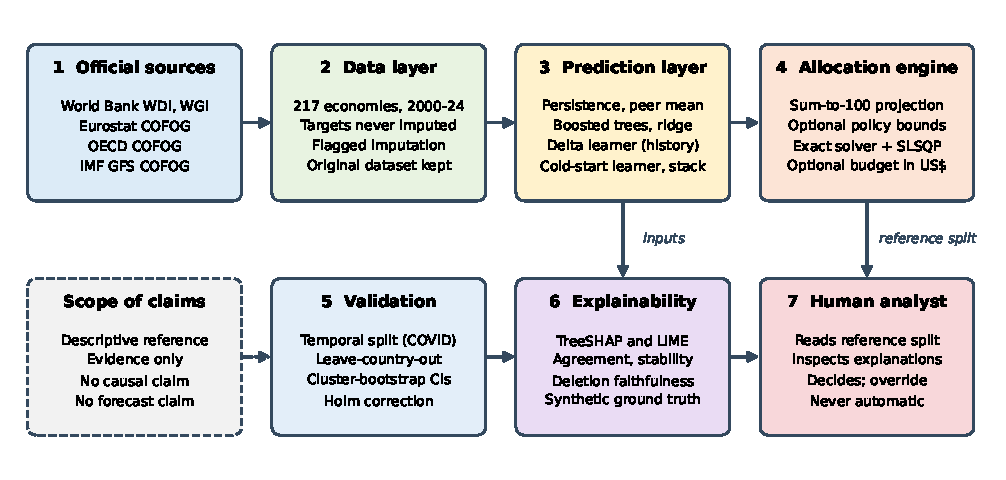
\includegraphics[width=0.85\textwidth]{figures/fig1_architecture.pdf}
\caption{Evaluated components of GovAllocXAI: official sources, flagged data layer, history-based and cold-start learners, bounded-simplex projection, explanation and validation layers; the intended user is a human analyst.}\label{fig:arch}
\end{figure*}}
\newcommand{\figAudit}{\begin{figure*}[!t]
\centering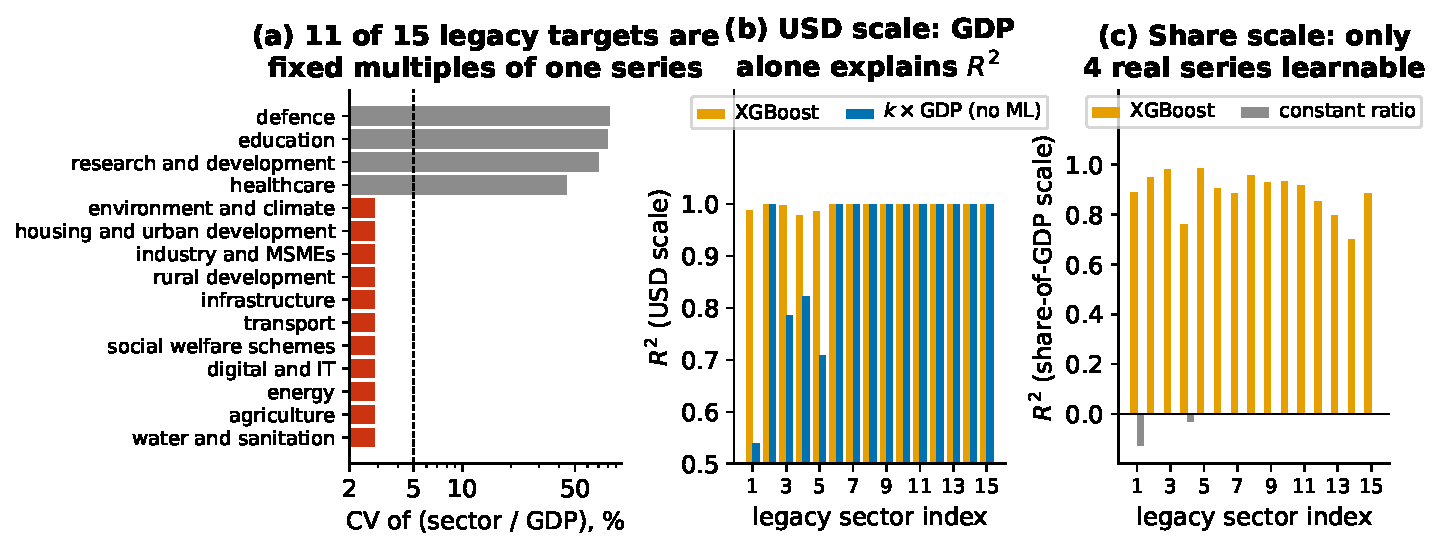
\includegraphics[width=\textwidth]{figures/fig3_legacy_audit.pdf}
\caption{Forensic audit of the legacy v1 benchmark: (a) eleven sectors are fixed multiples of one series; (b) $k\times$GDP matches XGBoost on them (USD scale); (c) a constant-share predictor has $R^2\approx0$ (share scale).}\label{fig:audit}
\end{figure*}}
\newcommand{\figMain}{\begin{figure*}[!t]
\centering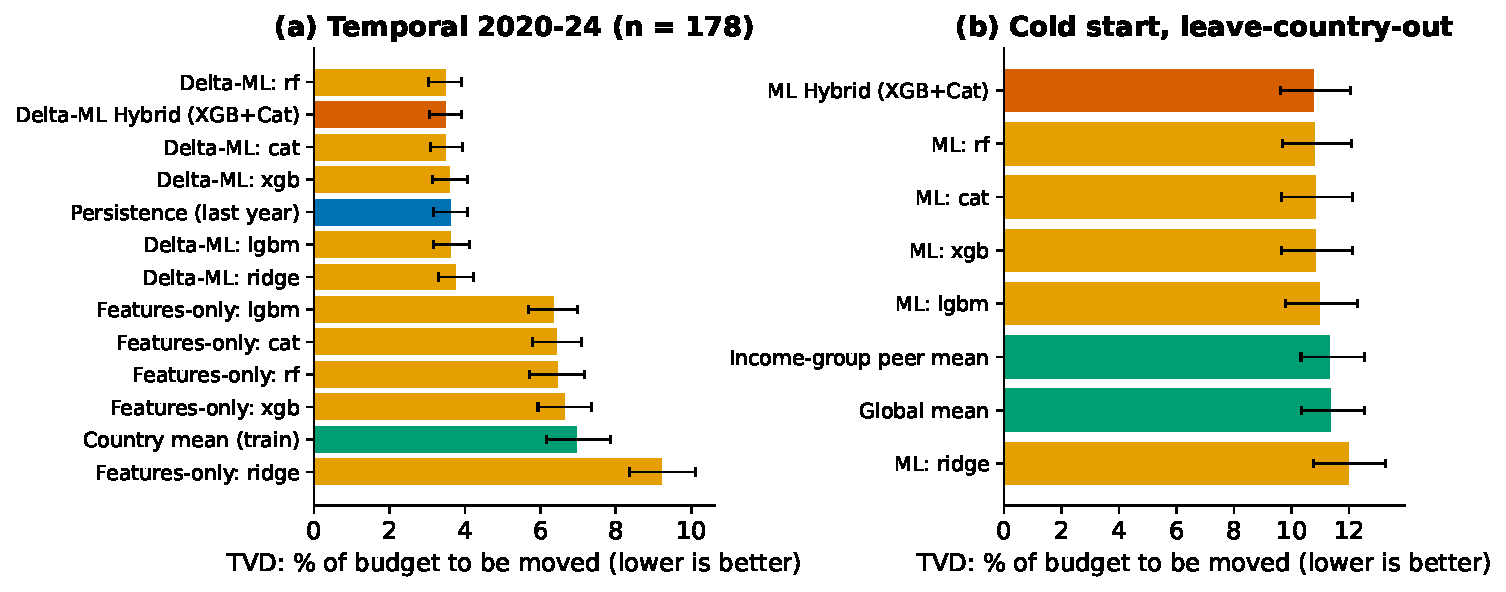
\includegraphics[width=\textwidth]{figures/fig4_main_results.pdf}
\caption{TVD on panel A16 with 95\% cluster-bootstrap CIs: (a) annual update (test 2020--24, $n=178$); (b) cold start (two fold seeds).}\label{fig:main}
\end{figure*}}
\newcommand{\figLime}{\begin{figure*}[!t]
\centering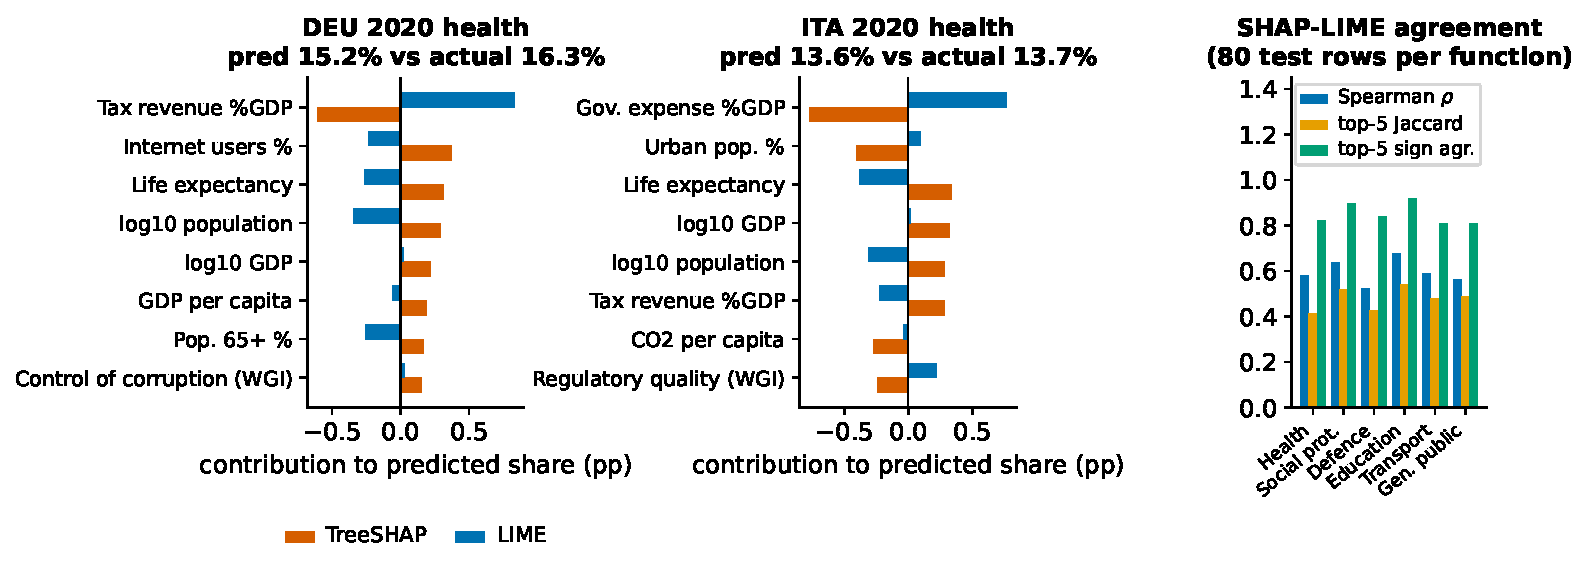
\includegraphics[width=\textwidth]{figures/fig8_shap_vs_lime.pdf}
\caption{SHAP vs.\ LIME: two case studies (signed contributions) and agreement metrics over 80 test rows per function.}\label{fig:lime}
\end{figure*}}
